\documentclass[]{beamer}
%\documentclass[handout]{beamer}
%\documentclass[handout,draft]{beamer}

% Preambulo
% Paquetes para usar bien el idioma español
\usepackage[spanish,es-tabla]{babel}
\selectlanguage{spanish}
\usepackage[utf8]{inputenc}

% Paquetes para usar mejores imagenes
\usepackage{graphicx}

% Paquetes para links y tabla de contenidos en el PDF
\usepackage{hyperref}
\hypersetup{colorlinks=true,allcolors=blue}
%\usepackage{hypcap}

% Paquetes para mejores tablas
\usepackage{booktabs}

% Mejor matematica
\usepackage{amsmath}

% Fuentes de las imagenes
\usepackage[absolute,overlay]{textpos}

% Paquete captions
\usepackage[justification=centering,labelformat=empty,labelsep=none]{caption}

% Opciones para ticks
\usepackage{tikz}
\usetikzlibrary{shapes,arrows,positioning}

\tikzstyle{decision} = [diamond, draw, fill=blue!20, text width=4em, text badly centered, node distance=2cm, inner sep=0pt,on grid]
\tikzstyle{block} = [rectangle, draw, fill=blue!20, text width=8em, text centered, rounded corners, minimum height=2em,on grid]
\tikzstyle{line} = [draw, -latex]

% Citas bibliograficas
\usepackage[backend=biber]{biblatex}
\renewcommand{\footnotesize}{\tiny}
\addbibresource{biblio.bib}

% Mejoro las captions
\setbeamertemplate{caption}{\raggedright\insertcaption\par}

\setbeamertemplate{caption}{%
\begin{beamercolorbox}[wd=0.85\paperwidth, sep=.2ex]{block body}\insertcaption%
\end{beamercolorbox}%
}


% Sacar barra de navegacion
\setbeamertemplate{navigation symbols}{}%remove navigation symbols

% Transparencias en items
\setbeamercovered{transparent}

% Estilo de diapositivas
% \usetheme{Boadilla}
\usecolortheme{whale}
\usecolortheme{orchid}


\title{Herramientas de Teledetección Cuantitativa\\{\small Clase 6}}
\author{Francisco Nemi\~na}
\institute{Unidad de Educación y Formación Masiva \\ Comisión Nacional de
Actividades Espaciales}
%\institute[Inst.]{
\includegraphics[height=1cm]{Figures/logosopi.png}\phantom{pepe} 
\includegraphics[height=1cm]{Figures/2mp.png}\phantom{pepe} 
\includegraphics[height=1cm]{Figures/conae.png}}
\date{}
%\titlegraphic{
%\includegraphics[height=1cm]{IMAGENES/minplan.png}\phantom{1}
%
\includegraphics[height=1cm]{IMAGENES/conae.png}\phantom{1}
%
\includegraphics[height=1cm]{IMAGENES/sopi.png}}

\logo{
\includegraphics[height=0.7cm]{imagenes/sopi.png}}

\AtBeginSection[]
{
\begin{frame}
\frametitle{Esquema de presentación}
\tableofcontents[currentsection]
\end{frame}
}


\begin{document}
\begin{frame}
    \maketitle
\end{frame}

\section{Matemática}
\subsection{Estadística}
\begin{frame}{\subsecname}
  \begin{block}{Notación}
    Notamos a la media para la clase $\omega_i$ como $$m_i = \frac{1}{q_i-1} \sum_j^{q_i} x_j$$ donde $q_i$ es la cantidad de píxeles de la clase.
  \end{block}\pause
  \begin{block}{Notación}
    La varianza como $$\sigma_i^2 = \frac{1}{q_i-1} \sum_j^{q_i} (x_j-m_i)^2$$ dónde los $x_j$ pertenecen a la clase $i$.
  \end{block}
\end{frame}
%--- Next Frame ---%

\begin{frame}{\subsecname}
  \begin{block}{Probabilidad condicional}
    Recordamos a la probabilidad condicional como $$p(x|\omega_i)$$ como la probabilidad de encontrar a un píxel en el punto $x$ del espacio espectral dado que sabemos que pertenece a la clase $\omega_i$.
  \end{block}
\end{frame}
%--- Next Frame ---%

\begin{frame}{\subsecname}
  \begin{block}{Teorema de Bayes}
    $$p(\omega_i|x) = \frac{p(x|\omega_i) p(\omega_i)}{p(x)}$$
    Es decir, la probabilidad de que un píxel pertenezca a la clase $\omega_i$ dado que se encuentra en el punto del espacio espectral $x$.
  \end{block}
\end{frame}
%--- Next Frame ---%

\begin{frame}{\subsecname}
  \begin{block}{Distribución de Gauss multidimensional}
    Si definimos a la matriz de covarianza como $$C_i = \frac{1}{q_i-1} \sum_j^{q_i} (x_j-m_i)(x_j-m_i)^T$$ podemos definir la distribución de Gauss en un espacio multidimensional como $$p(x|\omega_i) \sim \exp (\frac{-1}{2} (x-m_i)^T C_i^{-1} (x-m_i) )$$
  \end{block}
\end{frame}
%--- Next Frame ---%

\section{Clasificación supervisada}
\subsection{Idea}
\begin{frame}{Motivación}
  \begin{center}
      \resizebox{0.4 \linewidth}{!}{%
        \begin{tikzpicture}[node distance = 2cm, auto]
          \node[block]                                (init) {Firma Espectral};\pause
          \node[block, below= of init]                (resp) {Reflectancia Espectral Efectiva};
          \path[line] (init) --          (resp);
          \pause
          \node[block, below= of resp]             (ques) {Categorías};
          \path[line] (resp) --          (ques);\pause
        \end{tikzpicture}%
      }%
    \end{center}
\end{frame}
%--- Next Frame ---%

\begin{frame}{\subsecname}
  \begin{alertblock}{Importante}
    Ahora tenemos que definir apriori cuales son las clases que queremos y como encontrarlas.
  \end{alertblock}
\end{frame}
%--- Next Frame ---%

\begin{frame}{\subsecname}
  \begin{figure}
  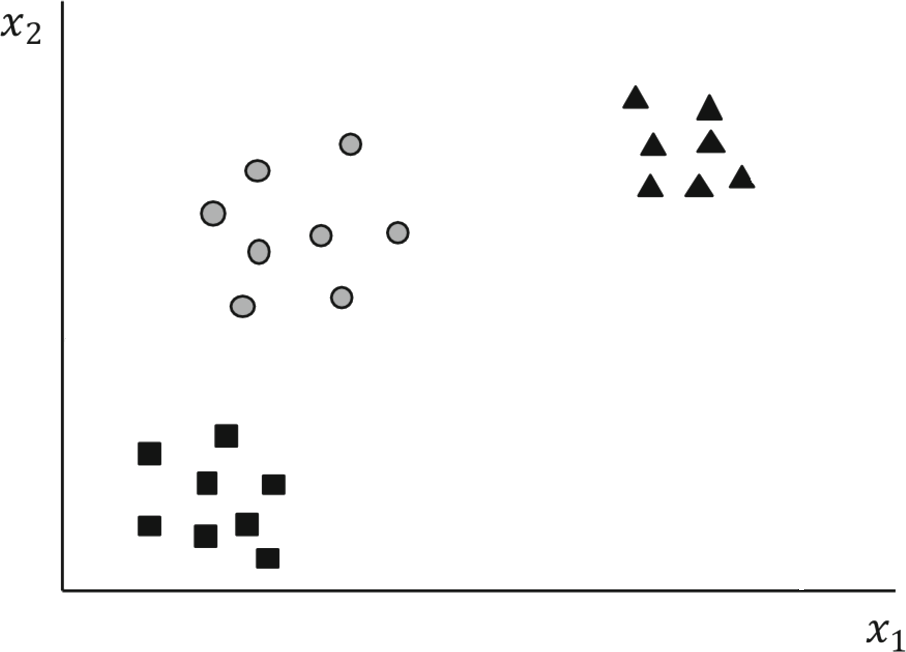
\includegraphics[width=0.6\textwidth]{imagenes/vector-3.png}
  \caption{Espacio vectorial.\footfullcite{richards2013remote}}
  \end{figure}
\end{frame}
%--- Next Frame ---%

\begin{frame}{\subsecname}
  \begin{figure}
  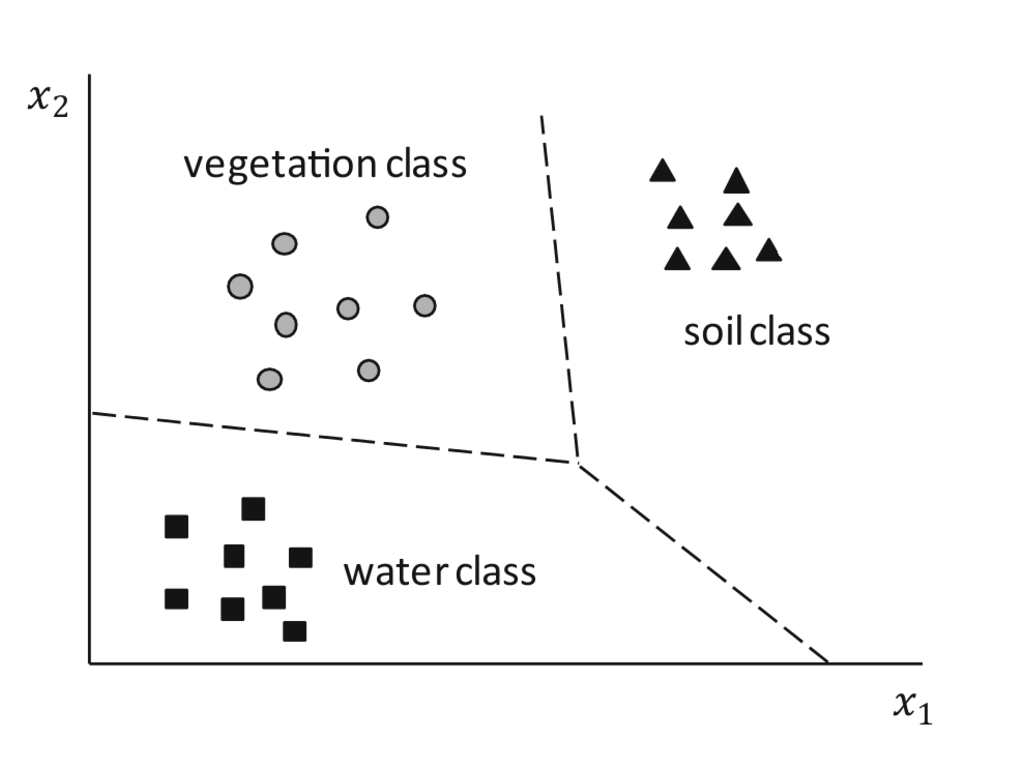
\includegraphics[width=0.6\textwidth]{imagenes/vector-2.png}
  \caption{Clasificación del espacio vectorial a partir de clases de entrenamiento.\footfullcite{richards2013remote}}
  \end{figure}
\end{frame}

\begin{frame}{\subsecname}
  \begin{block}{Esquema general}
    \begin{enumerate}[<+>]
      \item Decidir cuales son las clases de intereés.
      \item Elegir píxeles conocidos y representativos para cada clase a utilizar como áreas de entrenamiento.
      \item Estimar los parámetros del método de clasificación.
      \item Usar el clasificador para clasificar los pixeles.
      \item Producir mapas temáticos para extraer información.
      \item Corroborar la precisión de la clasificación con datos de campo
    \end{enumerate}
  \end{block}
\end{frame}
%--- Next Frame ---%

%--- Next Frame ---%
\subsection{Métodos}
\begin{frame}{\subsecname}
  \begin{block}{Generales}
    \begin{itemize}
      \item<.> Paralelepípedos
      \item<.> Distancia mínima
      \item<1> Máxima verosimilitud
      \item<.> Ángulo espectral
    \end{itemize}
  \end{block}
\end{frame}
%--- Next Frame ---%

\subsection{Máxima verosimilitud}

\begin{frame}{\subsecname}
  \begin{block}{Clasificador Bayesiano}
    Si conocemos las probabilidades condicionales $p(\omega_i|x)$ entonces un píxel $x$ pertenece a la clase $\omega_i$ si $$p(\omega_i|x)>p(\omega_j|x)$$ si $i \neq j$.
  \end{block}
  \pause
  \begin{alertblock}{Problema}
    No conocemos $p(\omega_i|x)$.
  \end{alertblock}
\end{frame}
%--- Next Frame ---%

\begin{frame}{\subsecname}
  \begin{block}{Solución}
    Usamos el teorema de Bayes y podemos escribir que un píxel $x$ pertenece a la clase $\omega_i$ si $$p(x|\omega_i)p(\omega_i)>p(x|\omega_j)p(\omega_j)$$ si $i \neq j$.
  \end{block}
  \pause
  \begin{block}{Función discriminante}
    Si definimos $g_i(x) = \log (p(x|\omega_i)p(\omega_i))$ entonces lo anterior se convierte en $x$ pertenece a la clase $\omega_i$ si $$g_i(x)>g_j(x)$$ si $i \neq j$.
  \end{block}
\end{frame}
%--- Next Frame ---%

\begin{frame}{\subsecname}
  \begin{block}{Caso Gaussiano}
    Si suponemos que la distribución $p$ es normal y que, apriori la probabilidad de pertenecer a una clase es equiprobable, tenemos que
    $$g_i(x) = -\log |C_i| - (x-m_i)^T C_i^{-1} (x-m_i)$$.
  \end{block}
  \pause
  \begin{alertblock}{Observaciones:}
    Como la distribución de Gauss no se anula nunca, esto puede clasificar a lo largo de todo el espacio
  \end{alertblock}
\end{frame}
%--- Next Frame ---%

\begin{frame}{\subsecname}
  \begin{block}{Superficies de equiprobabilidad}
    Si buscamos la superficies de $$g_i = g_j$$ ese espacio queda dividido en distintos sectores donde es siempre mayor la probabilidad de pertenecer a una clase.
    \pause
    Son
    \begin{itemize}[<+>]
      \item Elipses
      \item Parábolas
      \item Hipérbolas
    \end{itemize}
  \end{block}
\end{frame}
%--- Next Frame ---%

\begin{frame}{\subsecname}
  \begin{figure}
  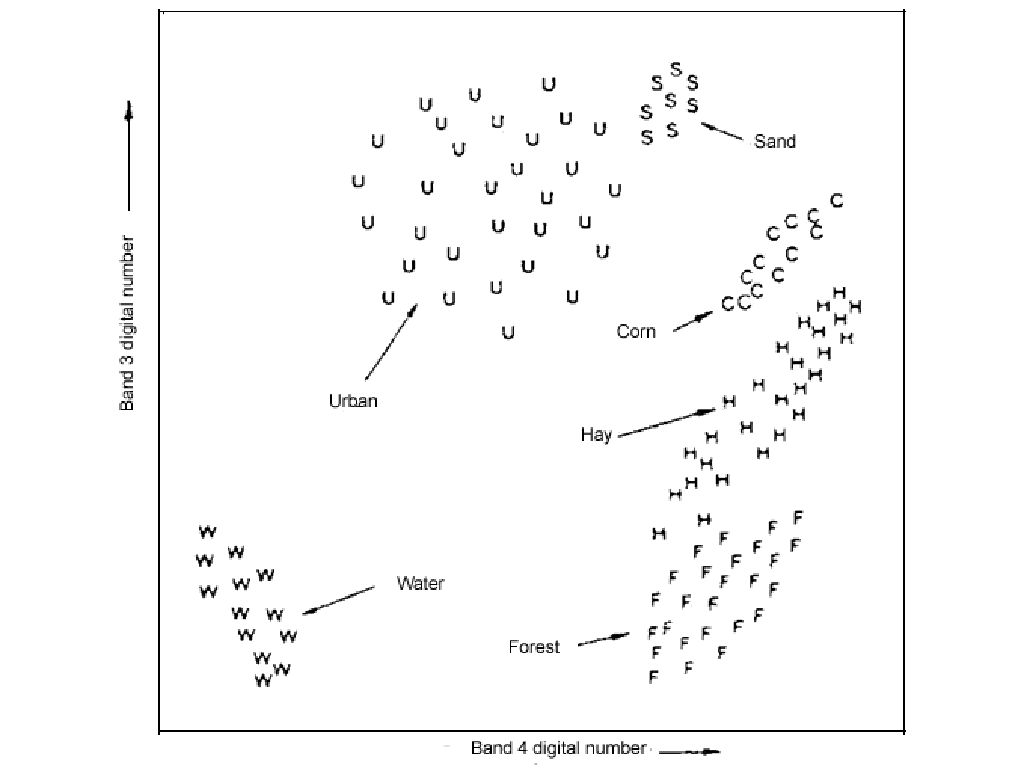
\includegraphics[width=0.6\textwidth]{imagenes/areas.png}
  \caption{Vista en el espacio vectorial.\footfullcite{clasif1}}
  \end{figure}
\end{frame}
%--- Next Frame ---%

\begin{frame}{\subsecname}
  \begin{figure}
  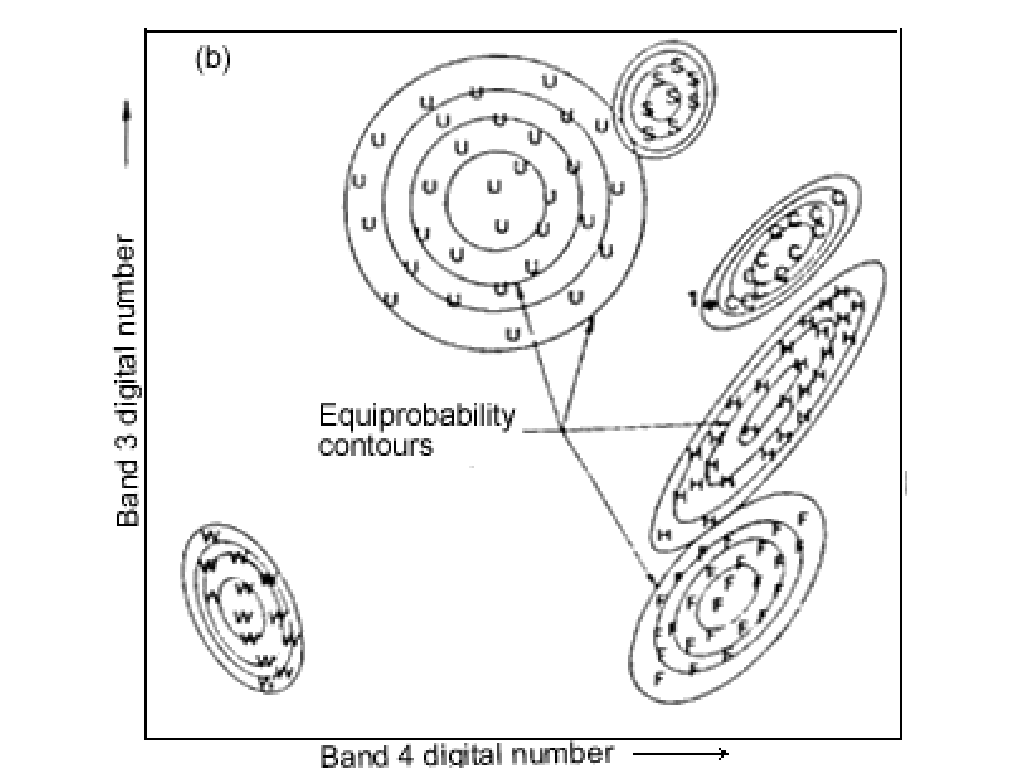
\includegraphics[width=0.6\textwidth]{imagenes/max.png}
  \caption{Vista en el espacio vectorial.\footfullcite{clasif1}}
  \end{figure}
\end{frame}
%--- Next Frame ---%

\begin{frame}{\subsecname}
  \begin{block}{Número de píxeles necesarios}
    Para estimar la matriz de covarianza se necesitan al menos $N(N+1)$ elementos. Es decir, al menos $N+1$ píxeles.
  \end{block}
\end{frame}
%--- Next Frame ---%

\begin{frame}{\subsecname}
  \begin{figure}
  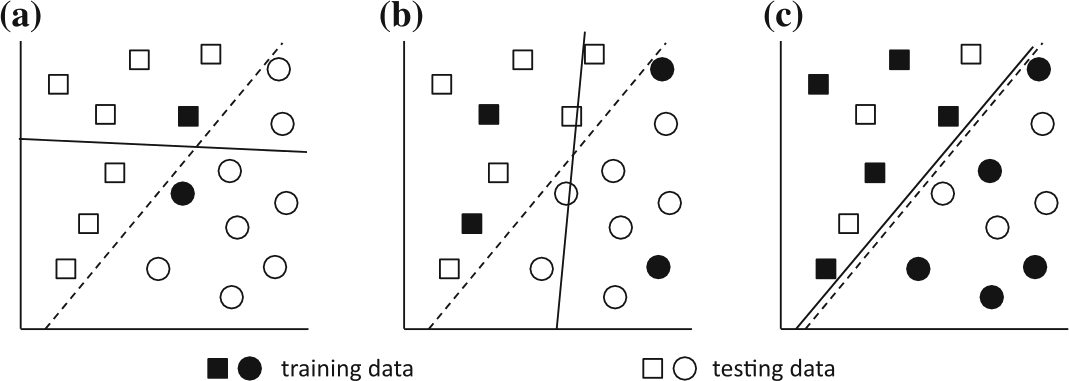
\includegraphics[width=0.8\textwidth]{imagenes/train.png}
  \caption{Clasificación supervisada incrementando el número de píxeles de entrenamiento.\footfullcite{richards2013remote}}
  \end{figure}
\end{frame}
%--- Next Frame ---%

\begin{frame}{\subsecname}
  \begin{alertblock}{Número de píxeles necesarios}
    En la práctica, se necesitan entre $10N$ y $100N$ píxeles.
  \end{alertblock}
\end{frame}
%--- Next Frame ---%

\begin{frame}{\subsecname}
  \begin{figure}
  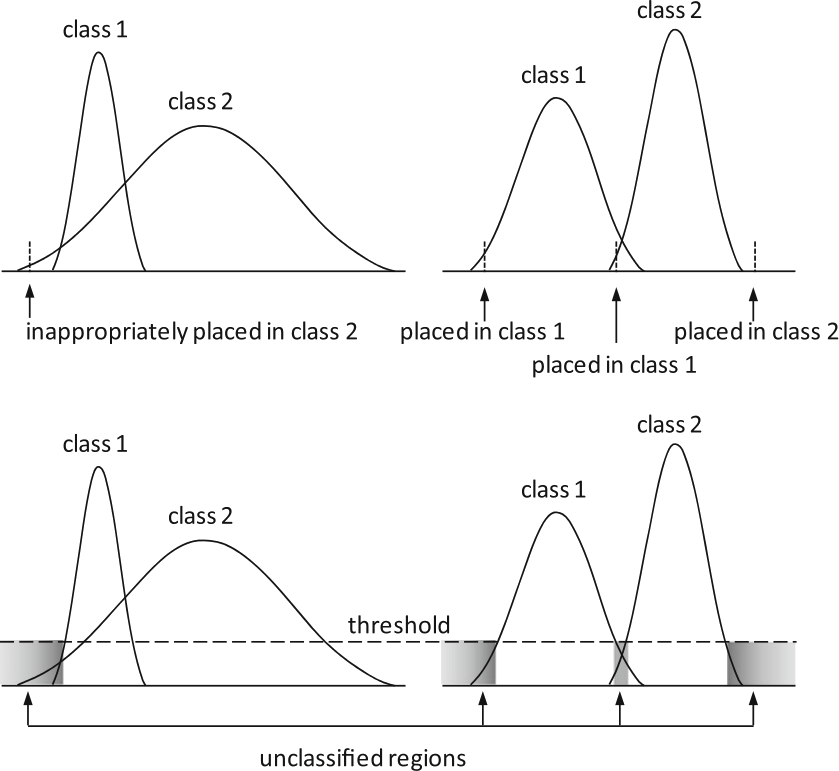
\includegraphics[width=0.6\textwidth]{imagenes/thresh.png}
  \caption{Problemas de clasificación y umbral.\footfullcite{richards2013remote}}
  \end{figure}
\end{frame}
%--- Next Frame ---%

\begin{frame}{\subsecname}
  \begin{figure}
  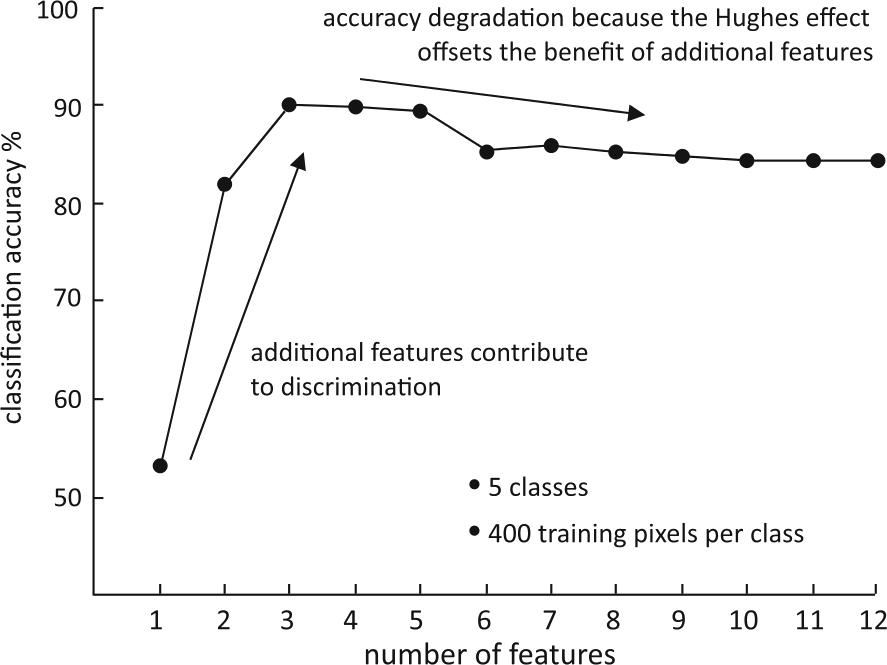
\includegraphics[width=0.8\textwidth]{imagenes/hughes.png}
  \caption{Otro problema, fenómeno de Hughes.\footfullcite{richards2013remote}}
  \end{figure}
\end{frame}
%--- Next Frame ---%

\begin{frame}{\subsecname}
  \begin{figure}
  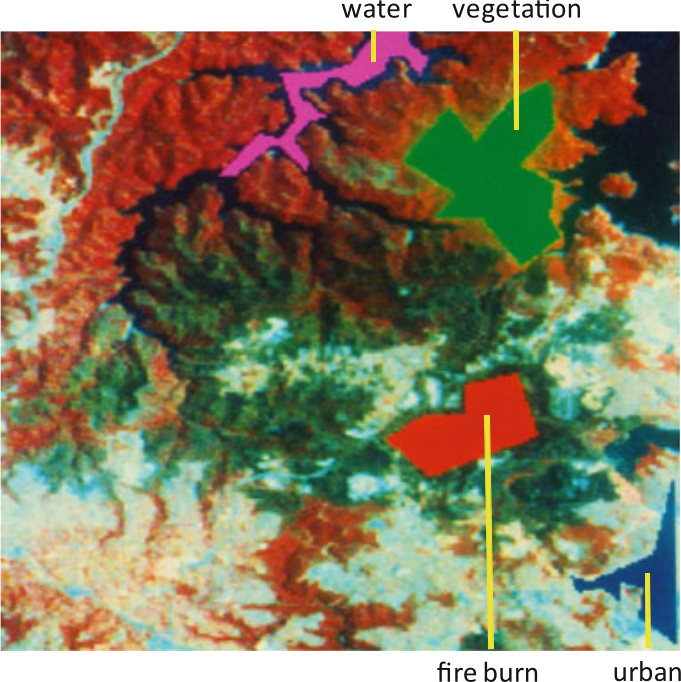
\includegraphics[width=0.6\textwidth]{imagenes/t_area.png}
  \caption{Imagen con áreas de entrenamineto.\footfullcite{richards2013remote}}
  \end{figure}
\end{frame}
%--- Next Frame ---%

\begin{frame}{\subsecname}
  \begin{figure}
  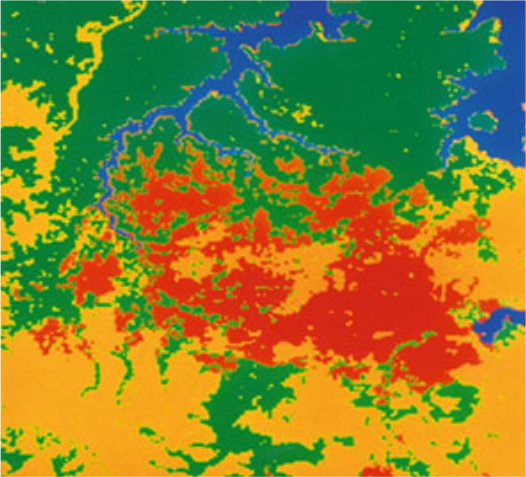
\includegraphics[width=0.6\textwidth]{imagenes/t_map.png}
  \caption{Imagen clasificada.\footfullcite{richards2013remote}}
  \end{figure}
\end{frame}
%--- Next Frame ---%

\subsection{Otros métodos}
\begin{frame}{\subsecname}
  \begin{block}{Pocos píxeles}
    Si contamos con pocos píxeles de entrenamiento, podemos caer en otros metodos.
    \begin{itemize}
      \item<.> Paralelepípedos
      \item<1> Distancia mínima
      \item<.> Máxima verosimilitud
      \item<1> Ángulo espectral
    \end{itemize}
  \end{block}
\end{frame}
%--- Next Frame ---%

\begin{frame}{\subsecname}
  \begin{block}{Distancia mínima}
    Si buscamos la superficies de $g_i = g_j$ con $g_i = 2 m_i x - m_i m_i$
    y me divide a mi espacio por hiperplanos.
  \end{block}
\end{frame}
%--- Next Frame ---%

\begin{frame}{\subsecname}
  \begin{figure}
  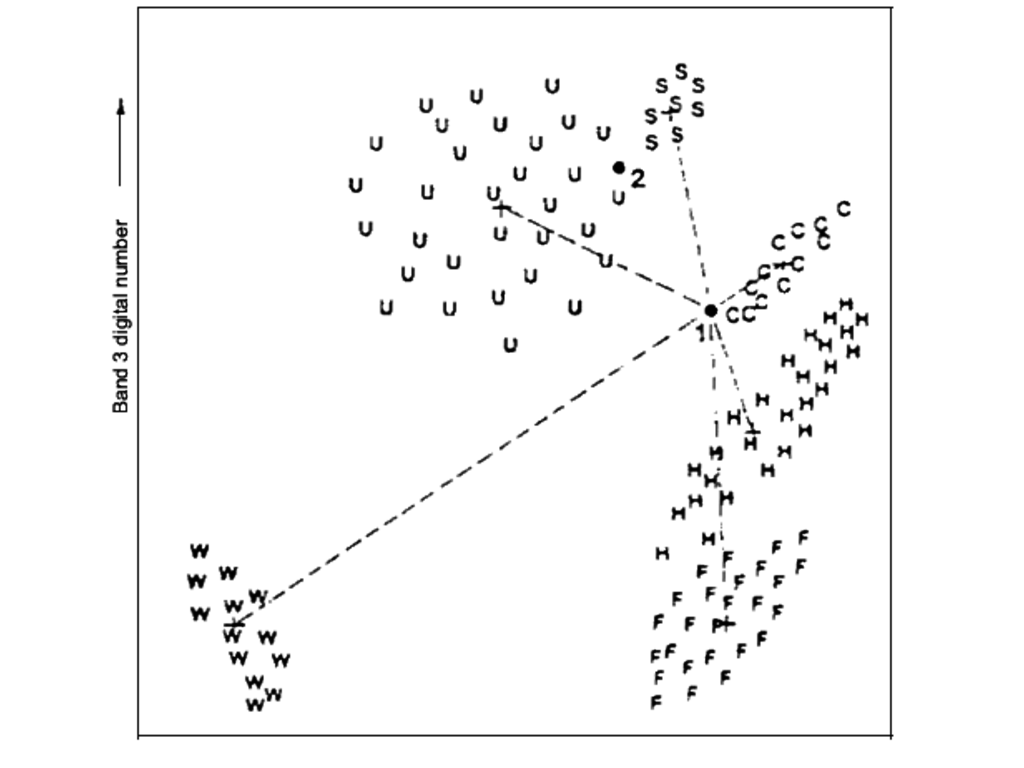
\includegraphics[width=0.6\textwidth]{imagenes/min.png}
  \caption{Vista en el espacio vectorial.\footfullcite{clasif1}}
  \end{figure}
\end{frame}
%--- Next Frame ---%

\begin{frame}{\subsecname}
  \begin{block}{Angulo espectral}
    Dividimos en este caso al espacio utilizando el ángulo correspondiente a los píxeles de entrenamiento.
  \end{block}
\end{frame}
%--- Next Frame ---%

\begin{frame}{\subsecname}
  \begin{figure}
  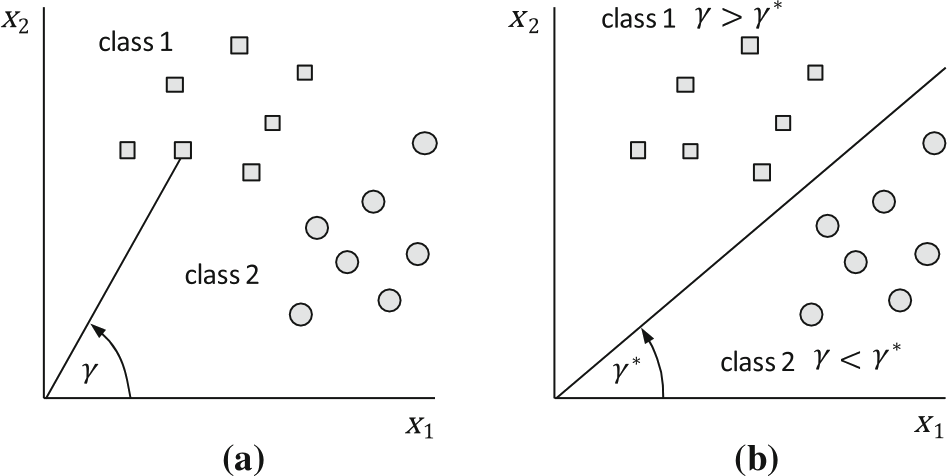
\includegraphics[width=0.6\textwidth]{imagenes/angle.png}
  \caption{Vista en el espacio vectorial.\footfullcite{richards2013remote}}
  \end{figure}
\end{frame}
%--- Next Frame ---%

\section{Práctica}

\begin{frame}{\secname}
  \begin{exampleblock}{Actividades prácticas de la cuarta clase}
    \begin{enumerate}[<+>]
      \item Abra las imágenes Landsat 8 y digitalice las coberturas de interés.
      \item Clasifique la imagen utilizando un vector de entrenamiento por clase.
      \item Clasifique la imagen utilizando varios vectores de entrenamiento por clase.
      \item Utilizce la herramienta de estadísticas globales para estimar las áreas correspondientes a cada uso y cobertura.
    \end{enumerate}
  \end{exampleblock}
\end{frame}
%--- Next Frame ---%

\end{document}
